%-------------------------------%
% Biblography
%------------------------------%
\RequirePackage{filecontents}        % loading package filecontents
% writing file \jobname.bib, for example mb-bibtex.bib.

\begin{filecontents*}{\jobname.bib}

@conference{,
%[A]
%[B]
@book{Bishop:06,
  title={Pattern recognition and machine learning},
  author={Christopher M Bishop},
  year={2006},
  publisher={Springer New York}
}

%[D]
@inproceedings{Das:08,
  title={Adapting to a Market Shock: Optimal Sequential Market-Making.},
  author={Das, Sanmay and Magdon-Ismail, Malik},
  booktitle={NIPS},
  pages={361--368},
  year={2008}
}
%[E]
%[F]
%[G]
%[H]
%[I]
%[J]
%[K]
@book{Keeney:93,
  title={Decisions with multiple objectives: preferences and value trade-offs},
  author={Keeney, Ralph L and Raiffa, Howard},
  year={1993},
  publisher={Cambridge university press.}% Original publication, Wiley, New York, 1976}
}

@book{Koller:09,
  title={Probabilistic graphical models: principles and techniques},
  author={Koller, Daphne and Friedman, Nir},
  year={2009},
  publisher={The MIT Press}
}
%[L]
%[N]
%[O]
%[P]
%[Q]
%[R]
%[S]
@conference{Sanner:12,
author = {Scott Sanner and Ehsan Abbasnejad},
title = {Symbolic Variable Elimination for Discrete and Continuous Graphical Models},
booktitle = {AAAI},
year = {2012}
}
%[T]
%[U]
%[V]
%[W]
%[X]
%[Y]
%[Z]

\end{filecontents*}

\documentclass{article} % For LaTeX2e
\usepackage{nips13submit_e,times}%{nips13submit_e,times}
\usepackage{hyperref}
\usepackage{url}
\usepackage{amsthm} %for theorems, examples, etc.
\usepackage{amsfonts} %for matbb font
\usepackage{graphicx}
\usepackage{caption} %for graphics
\usepackage{subcaption} %for graphics
\usepackage{amsmath} %for cases

\usepackage{algorithmic} %for algorithms
% Import an algorithm formatting package
\usepackage[vlined,algoruled,titlenumbered,noend]{algorithm2e}
%\documentstyle[nips13submit_09,times,art10]{article} % For LaTeX 2.09
%\usepackage{algpseudocode} %new tpr
%\usepackage{algorithm} %new tpr

\usepackage{verbatim} %for commenting

%\newenvironment{proof}{{\noindent\bf Proof.}}\qed%{\hspace*{\fill}\ensuremath{\diamondsuit\quad}%{\vskip 1ex}
\newtheorem{theorem}{Theorem}
\newtheorem{proposition}{Proposition}
\newtheorem{example}{Example}
\def\fexample#1#2#3{\vspace{-1ex}\begin{example}[#2]\label{#1}\rm #3
\hspace*{\fill} $\diamondsuit\quad$ \end{example}\vspace{-2ex} }
\newcommand{\tuple}[1] {\langle #1 \rangle}
\newcommand{\bvec}[1]{\textbf{#1}}
\newcommand{\indicator}{\mathbb{I}}%{I\!\!I}

\def\eqvsp{}  \newdimen\paravsp  \paravsp=1.3ex
\def\paradot#1{\vspace{\paravsp plus 0.5\paravsp minus 0.5\paravsp}\noindent{\bf\boldmath{#1.}}}

\title{
%Blocked Gibbs Sampling on Piecewise Bayesian Networks
Fast Bayesian Inference in Piecewise Graphical Models
}


\author{
%David S.~Hippocampus\thanks{ Use footnote for providing further information
%about author (webpage, alternative address)---\emph{not} for acknowledging
%funding agencies.} \\
%Department of Computer Science\\
%Cranberry-Lemon University\\
%Pittsburgh, PA 15213 \\
%\texttt{hippo@cs.cranberry-lemon.edu} \\
%\And
%Coauthor \\
Affiliation \\
Address \\
\texttt{email} \\
\AND
Coauthor \\
Affiliation \\
Address \\
\texttt{email} \\
\And
Coauthor \\
Affiliation \\
Address \\
\texttt{email} \\
\And
Coauthor \\
Affiliation \\
Address \\
\texttt{email} \\
(if needed)\\
}

% The \author macro works with any number of authors. There are two commands
% used to separate the names and addresses of multiple authors: \And and \AND.
%
% Using \And between authors leaves it to \LaTeX{} to determine where to break
% the lines. Using \AND forces a linebreak at that point. So, if \LaTeX{}
% puts 3 of 4 authors names on the first line, and the last on the second
% line, try using \AND instead of \And before the third author name.

\newcommand{\fix}{\marginpar{FIX}}
\newcommand{\new}{\marginpar{NEW}}

%\nipsfinalcopy % Uncomment for camera-ready version

\begin{document}

\maketitle

\begin{abstract}
%In many real world probabilistic inference tasks such as \emph{preference learning}, predicting traders behaviors in a financial market, etc. prior/likelihood models are intrinsically piecewise. This work shows that Gibbs sampling can effectively be used on piecewise linear/quadratic polynomial distributions. It happens that in a Bayesian model,  the number of partitions in the \emph{posterior} distribution can grow exponentially if the \emph{likelihood} is piecewise. A major contribution is to show that such networks can be regarded to as mixture models leading to a computation reduction which is exponential to linear in the amount of data. We provide a Blocked Gibbs sampling algorithm which is quite effective on such models. The empirical results show that the performance of this sampling method is order of magnitudes better than candidate algorithms for asymptotically unbiased reasoning. The generalization of the proposed sampling method to any piecewise distribution with a huge number of partitions is straight forward. 
Many real-world Bayesian inference problems such as preference learning, competitive skill learning, and Bayesian belief updating with state constraints naturally use piecewise transitions, likelihoods or prior models. Unfortunately, exact closed-form inference in these graphical models is intractable in the general case and existing approximation techniques provide few guarantees on both approximation quality and efficiency. While (Markov Chain) Monte Carlo sampling provides an attractive asymptotically unbiased approximation approach, rejection sampling and Metropolis-Hastings both prove inefficient in practice, and analytical derivation of Gibbs samplers require exponential space and time in the amount of data or other quantities relating to graphical model size. 
In this work, we show how to convert piecewise graphical models to equivalent mixture models and then use  a blocked Gibbs sampling on the derived (\emph{augmented}) models. This algorithm achieves an exponential-to-linear reduction in space and time compared to a standard Gibbs sampler. This enables fast, asymptotically unbiased inference in a new expressive class of piecewise graphical models. 
\end{abstract}

\section{Introduction}
Many real world Bayesian inference problems such as preference learning, predicting traders’ behavior in a financial market, competitive skill learning, etc. naturally have piecewise likelihood and/or prior models. To date tools for carrying out Bayesian reasoning in such models are either approximate (namely, approximate message passing with Gaussian priors/posteriors) or unscalable. The latter group consists of sampling-based methods limited to Metropolis-Hastings and rejection sampling. They are considered unscalable since in many models their convergence rate is slow (in time). 
This is particularly true if they are not tunned well, in the sense that 
a ``proper" \emph{envelope distribution} (or \emph{proposal distribution}) 
which is required for rejection sampling (resp. Metropolis-Hasting sampling) is not chosen.
In practice, such a tunning can be difficult and problem-dependent. 
Gibbs sampling, on the other hand, does not require tunning, and in this sense, is robust.
Nonetheless, in piecewise models and in particular when likelihood models are piecewise,
the time/space computation costs of Gibbs sampling can grow exponential in the amount of observed data.    This is prohibitively expensive 
and to our knowledge, so far, Gibbs sampling has not been used in the aforementioned models. 

Our work fills this gap by providing a Bayesian inference method which is both scalable and asymptotically unbiased that can be used in a large family of piecewise models. 
In particular, the presented method reveals its superiority over the existing tools where the number of partitions in a piecewise distribution is huge.    

To motivate the need for piecewise models, consider the following running example:
%the following \emph{Bayesian preference learning} scenario is used as a concrete running example throwout:
%%%%%%%%%%%%%%%%%%%%%%%%%
\begin{figure}%[t!]
\centering
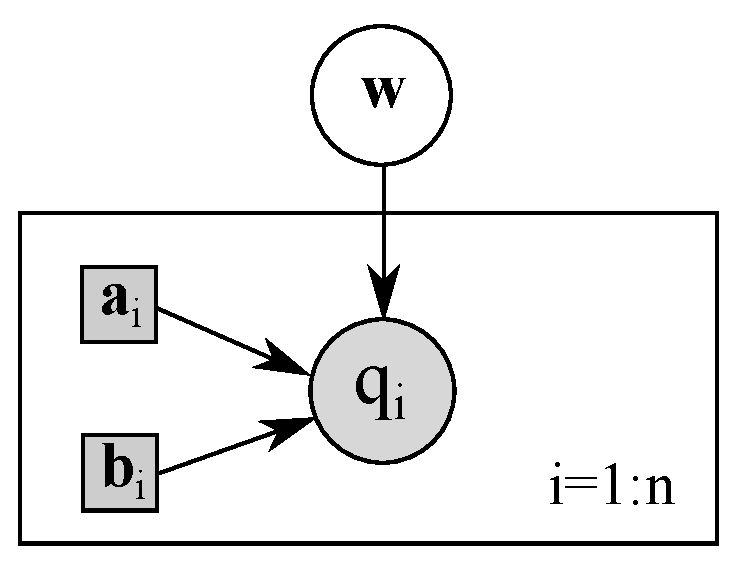
\includegraphics[width=.29\textwidth]{pic/pref2.pdf}
%\vspace{-6mm}
\caption{\footnotesize Graphical model for BPPL problem in Example \ref{example:pref}. }
\label{fig:pref}
%\caption{\footnotesize .} 
%\vspace{4mm}
\end{figure}
%%%%%%%%%%%%%%%%%%%%%%%%%
%%%%%%%%%%%%%%%%%%%%%%%%%
\begin{figure}
\centering
\begin{subfigure}{.45\textwidth}
  \centering
  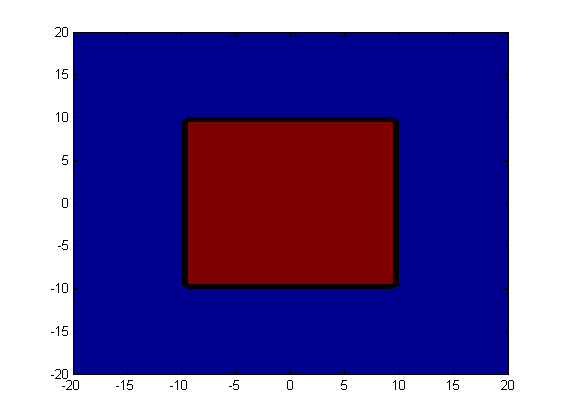
\includegraphics[width=.5\textwidth]{pic/prior2d.png}
  \caption{}
  \label{fig:prior2d}
\end{subfigure}%
\begin{subfigure}{.45\textwidth}
  \centering
  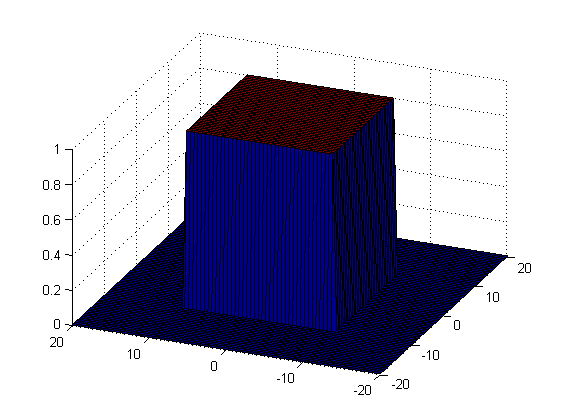
\includegraphics[width=.5\textwidth]{pic/prior3d.png}
  \caption{}
  \label{fig:prior3d}
\end{subfigure}
\begin{subfigure}{.45\textwidth}
  \centering
  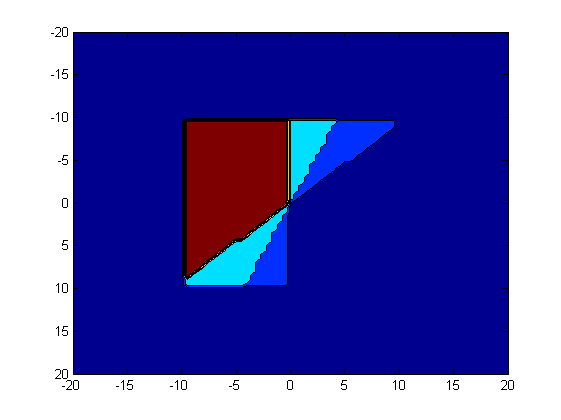
\includegraphics[width=.5\textwidth]{pic/posterior2d.png}
  \caption{}
  \label{fig:posterior2d}
\end{subfigure}%
\begin{subfigure}{.45\textwidth}
  \centering
  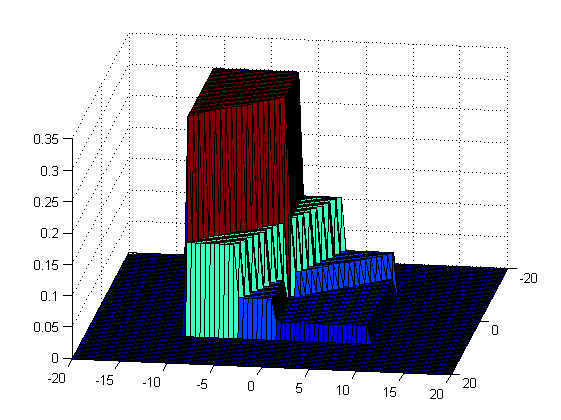
\includegraphics[width=.5\textwidth]{pic/posterior3d.png}
  \caption{}
  \label{fig:posterior3d}
\end{subfigure}
\caption{\footnotesize Prior/posterior distribution of the parameter vector $\bvec{w}$ of Example \ref{example:pref} in a 2D feature space.
(a) \& (b) A 2D/3D representation of uniform prior distribution $pr (\bvec{w})$.
(c) \& (d) The corresponding posterior distribution of $\bvec{w}$ given 3 user preference query responses.}
\label{fig:prior}
\end{figure}
%%%%%%%%%%%%%%%%%%%%%%
\fexample{example:pref}{Bayesian pairwise preference learning (BPPL)}{
Suppose each \emph{item} $\bvec{a}$ is an $N$-dimensional real-valued \emph{attribute choice vector} 
$(\alpha_1, \ldots, \alpha_N)$.
The goal is to learn an \emph{attribute weight vector} 
$\bvec{w} = (w_1, \ldots, w_N) \in \mathbb{R}^N$ (with prior distribution being uniform in a $N$ dimensional hyperrecangle)
that describes the utility of each attribute choice from user responses to preference queries.
As commonly done in \emph{multi-attribute utility theory} \cite{Keeney:93},
the overall item utility $u(\bvec{a}|\bvec{w})$ decomposes additively over the attribute choices of $\bvec{a}$:
%
$u(\bvec{a} | \bvec{w}) = \sum_{j=1}^N w_j \cdot \alpha_j$.\\
User responses are in the form of $n$ queries $q_1$ to $q_n$ where each query $q_i$ is a pairwise comparison of some items $\bvec{a}_i$ and $\bvec{b}_i$ with possible 
responses $\textsc{Val}(q_i) = \{\textsc{First}, \textsc{Second}\}$ where $q_i = \textsc{First}$ means $\bvec{a}_i$ is preferred over $\bvec{b}_i$ and 
$q_i = \textsc{Second}$ indicates the opposite. 
For the sake of simplicity, \emph{indifference} choice is not available. 
It is assumed that with an \emph{elicitation noise} $0 \leq \eta < 0.5$, the item with a greater overall utility is preferred:
\begin{equation*}
%\label{e:pref1likelihood}
pr(q_i = \textsc{First} \,|\, \bvec{w}, \bvec{a}_i, \bvec{b}_i) =
{\footnotesize
\begin{cases}
u(\bvec{a}_i|\bvec{w}) < u(\bvec{b}_i|\bvec{w}) : &\eta\\
u(\bvec{a}_i|\bvec{w}) = u(\bvec{b}_i|\bvec{w}) : &0.5\\
u(\bvec{a}_i|\bvec{w}) > u(\bvec{b}_i|\bvec{w}) : &1-\eta
\end{cases}
}%end footnote size
\end{equation*}
and $pr(q_i \!=\! \textsc{Second} \,|\, \bvec{w}, \bvec{a}_i, \bvec{b}_i) = 
1 - pr(q_i \!=\! \textsc{First} \,|\, \bvec{w}, \bvec{a}_i, \bvec{b}_i)$.
As the graphical model in Figure~(\ref{fig:pref}) illustrates:
$%begin{equation*}
pr(\bvec{w} | q_1, \bvec{a}_1, \bvec{b}_1, \ldots, q_n, \bvec{a}_n, \bvec{b}_n) 
\propto pr(\bvec{w}) \cdot \prod_{i=1}^{n} pr(q_i | \bvec{w}, \bvec{a}_i, \bvec{b}_i)
$.%end{equation*}
} %end example 1

\section{Graphical models}
\label{sec:graph_models}
A \emph{graphical model} is a diagrammatic representation of the conditional dependence structure between random variables. 
A \emph{Bayesian network} is a graphical model in form of a \emph{directed acyclic graph}
in which a factorization of the joint probability of all random variables $X_1,\ldots,X_n$ is represented as 
$pr(X_1,\ldots,X_n)=\prod_{i=1}^n pr \big( X_i | \, \textsc{Par}(X_i)\big)$, 
where $\textsc{Par}(X_i)$ is the set of parents of node $X_i$.
Although the inference method that will be presented in this paper can be used on 
any Bayesian network, for the sake of simplicity, we focus on \emph{Bayesian inference} 
on networks with the model illustrated in Figure~\ref{fig:naive} where a single \emph{parameter} (vector) $\boldsymbol\theta$
determines the distribution of data points $d_i$. 
Given a set of $n$ observed data points, 
the posterior distribution of $\boldsymbol\theta$ is simply computed as:
\begin{equation}
\label{e:posterior}
pr(\boldsymbol\theta | \, d_1, \ldots, d_n) 
\propto pr(\boldsymbol\theta) \cdot \prod_{i=1}^{n} pr(d_i | \boldsymbol\theta)
\end{equation} 
Example~\ref{example:pref} provides an instance of Bayesian inference in which the parameter is $\bvec{w}$
and observed data points are user preferences $q_1$ to $q_n$.
%%%%%%%%%%%%%%%%%%%%%%%%%
\begin{figure}
\centering
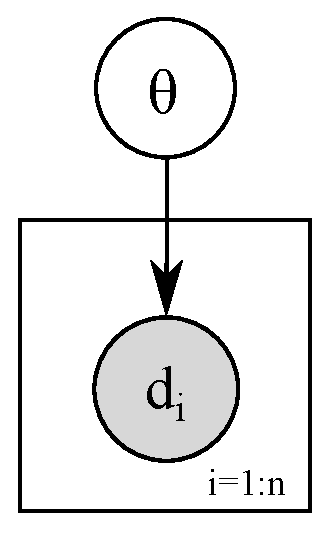
\includegraphics[width=0.16\textwidth]{pic/naive.pdf}
\caption{\footnotesize General Bayesian inference model with parameter $\boldsymbol\theta$ and data points $d_1$ to $d_n$ using \emph{plate notation}
(a plate groups variables that repeat together).
}
\label{fig:naive}
\end{figure}
%%%%%%%%%%%%%%%%%%%%%%%

\subsection{General piecewise models}
A function $f(\bvec{x})$ is called \emph{piecewise} if it can be represented in form of Relation~(\ref{e:piecewise}) where $\phi_1$ to $\phi_m$ are mutually exclusive and jointly exhaustive Boolean functions (constraints) 
that partition the space of variable(s) $\bvec{x}$. If for a particular variable assignment $\bvec{x}_0$, a constraint $\phi_i(\bvec{x}_0)$ is satisfied, then by definition, $f(\bvec{x}_0) = f_i(\bvec{x}_0)$.  
\begin{equation}
\label{e:piecewise}
f(\bvec{x}) = 
{\footnotesize
\begin{cases}
\phi_1(\bvec{x}) : & f_1(\bvec{x})\\
\vdots\\
\phi_m(\bvec{x}) : & f_m(\bvec{x})
\end{cases}
}%end footnote size
\end{equation}
In Example~\ref{example:pref}, BPPL is a \emph{piecewise constant} model
in the sense that both prior and likelihood models %(defined in relation ~\ref{e:pref1likelihood}) 
are piecewise and their corresponding \emph{sub-functions} ($f_i$) are constant.
A more general piecewise model where the sub-functions are not constant is presented in  Section~\ref{sect:experiment}. 



\section{Inference on Graphical models}
\label{sec:inference}
In theory, closed form inference on piecewise functions (at least piecewise polynomials) with linear constraints is possible \cite{Sanner:12}.
In practice, however, such symbolic methods rapidly become intractable. 
The second best option is to use methods which are \emph{asymptotically unbiased} (i.e.\ converge to the exact solution). The existing asymptotically unbiased inference tools are based on sampling.
Given a set of $S$ samples (particles) $\{\boldsymbol\theta^{(1)}, \ldots, \boldsymbol\theta^{(S)}\}$ taken from a posterior  distribution $pr(\boldsymbol\theta | \, d_1, \ldots, d_n)$, inference can be performed easily. 
For example, the posterior probability of an unobserved data point $d_{n+1}$, given by:
\[
pr(d_{n+1} | \, d_1, \ldots, d_n) = 
\int_{\boldsymbol\theta} pr(d_{n+1} | \, \boldsymbol\theta) pr(\boldsymbol\theta | \, d_1, \ldots, d_n) d\boldsymbol\theta 
\]
can be approximated by: $\frac{1}{S} \sum_{i=1}^S pr(d_{n+1} | \, \boldsymbol\theta^{(i)})$.
Three widely used sampling methods are:

\paradot{Rejection sampling}
In many cases, direct sampling from a distribution $f(\bvec{x})$ (such as the \emph{posterior} in Fig.~\ref{fig:posterior3d}) is difficult
but there is an alternative distribution $g(\bvec{x})$ (e.g.\ the \emph{prior} in Fig.~\ref{fig:prior3d})
from which samples can be taken efficiently and $f(\bvec{x})/g(\bvec{x})$ is bound by a constant $c>0$.
%$\sup_{\bvec{x}} \{ f(\bvec{x})/g(\bvec{x}) \} \leq c$.  
To take a sample from $f(\bvec{x})$ by means of \emph{rejection sampling}, 
a sample $\bvec{s}$ is taken from $g(\bvec{x})$ and accepted with probability $f(\bvec{s}) / c g(\bvec{s})$, 
otherwise it is rejected. In the latter case, the process is repeated. 
If $g(\bvec{x})$ is ``close" enough to $f(\bvec{x})$ (i.e.\ $c$ is close to 1), 
the sampling performance is high but if there is no known such distribution from which samples can be taken efficiently, the performance can be low 
since to accept a single sample, a huge amount of samples are typically rejected. 
%

\paradot{Metropolis-Hastings}
In this method in order to generate a new sample $\bvec{x}^{(t)}$ given a last obtained sample $\bvec{x}^{(t-1)}$ of a distribution $f(\bvec{x})$, 
firstly, a sample $\bvec{x}'$ is taken 
from a symmetric \emph{jumping distribution} $g(\bvec{x} |\, \bvec{x}^{(t-1)})$ (often a \emph{Gaussian} centered at $\bvec{x}^{(t-1)}$) from which samples can be taken efficiently. 
With probability $\min \big(1, f(\bvec{x}')/f(\bvec{x}^{(t-1)}) \big)$, 
$\bvec{x}'$ is accepted as the next sample (i.e.\ $\bvec{x}^{(t)} \leftarrow \bvec{x}'$)
otherwise, %but if $\bvec{x}'$ is rejected, 
$\bvec{x}^{(t)} \leftarrow \bvec{x}^{(t-1)}$. 
Choosing a \emph{jumping distribution} with `right' parameters is problem-dependent and requires extra tunning. An inappropriate \emph{jumping distribution} can lead to a slow convergence rate.
%

\paradot{Gibbs sampling}
In this method, to generate a new sample for a variable vector $\bvec{x} = (x_1, \ldots, x_N)$, 
each variable is sampled conditioned on the other variables being instantiated with their last sampled values:
$x_i \sim pr(x_i | x_{-i}^*)$. 
%In this method, to generate a sample $\bvec{x}^{(t)} = (x_1^{(t)}, \ldots, x_n^{(t)})$  of a distribution $f(\bvec{x})$ given a previous sample $\bvec{x}^{(t-1)}$, each $x_i^{(t)}$ is obtained by sampling conditioned on other variables i.e.\ from the conditional distribution $f(x_i | \, x_1^{(t)}, \ldots, \, x_{i-1}^{(t)} , \, x_{i+1}^{(t-1)}, \ldots, \, , \, x_{n}^{(t-1)})$. 
Unlike the other two methods, Gibbs sampling does not require any problem-dependent tunning. Nonetheless to generate a new particle vector, 
computation of $N$ \emph{cumulative distribution functions} (CDFs) 
(one for each $pr(x_i | x_{-i}^*)$) as well as their inverse functions is required which can be quite time consuming. 
Due to this shortcoming, in practice, Gibbs sampling can be prohibitively expensive.   

%
\subsection{Inference on piecewise models}\
As the following simple formula clarifies, 
the number of partitions in the product of two piecewise functions is equal to the product of the number of partitions in each of them:
\footnote{
If pruning potential inconsistent (infeasible) constraint is possible
(i.e.\ by \emph{linear constraint solvers} for linear constrains) and the imposed extra costs are justified,
the number of partitions can be less.
}%endfootnote
\[
{\footnotesize
\begin{cases}
\phi_1(\bvec{x}) : & f_1(\bvec{x})\\
\phi_2(\bvec{x}) : & f_2(\bvec{x})
\end{cases}
\otimes
\begin{cases}
\psi_1(\bvec{x}) : & g_1(\bvec{x})\\
\psi_2(\bvec{x}) : & g_2(\bvec{x})
\end{cases}
=
\begin{cases}
\phi_1(\bvec{x}) \wedge \psi_1(\bvec{x}) : & f_1(\bvec{x}) g_1(\bvec{x})\\
\phi_1(\bvec{x}) \wedge \psi_2(\bvec{x}) : & f_1(\bvec{x}) g_2(\bvec{x})\\
\phi_2(\bvec{x}) \wedge \psi_1(\bvec{x}) : & f_2(\bvec{x}) g_1(\bvec{x})\\
\phi_2(\bvec{x}) \wedge \psi_2(\bvec{x}) : & f_2(\bvec{x}) g_2(\bvec{x})
\end{cases}
}%end footnote size
\]
Therefore, in a Bayesian model with an $L$-piece prior and $n$ likelihoods each with at most $M$-piece,
the number of partitions in the posterior distribution is bounded
 by $LM^n$
i.e.\ the order of growth of the posterior's structural complexity is exponential in the amount of observed data. 

To perform Gibbs sampling on the posterior/joint distribution in a parameter space 
$\boldsymbol{\theta} = (\theta_1, \ldots, \theta_N)$,
for taking a single sample, $N$ number of CDFs should be computed (one for each paramter $\theta_i$ conditioned on the rest).
On the other hand, to compute each CDF,  up to $LM^n$ integration operations should be carried out
(one for each partition). Therefore, in total up to $LM^nN$ integration operations are required. This exponential growth rapidly makes Gibbs sampling intractable. 
The aim of this work is to make Gibbs sampling scalable by introducing a technique using which, this number can be reduced to $LM(N+n)$.

\section{Piecewise models as mixture models}
\label{sect:mix}
Consider a piecewise likelihood function:\footnote{
We concentrate exclusively on likelihood functions. However, Proposition~\ref{pro:discrete} can be applied to any piecewise distribution. 
}%footnote
\begin{equation}
\label{e:piecewise.likelihood22}
pr(d | \, \boldsymbol\theta) :=
{\footnotesize
\begin{cases}
\phi_1(\boldsymbol\theta)  &: f_1(\boldsymbol\theta, d)\\
\vdots\\
\phi_N(\boldsymbol\theta)  &: f_N(\boldsymbol\theta, d)
\end{cases}
}%end font size 
\end{equation} 
A simple but key observation is that since the constraints, $\phi_i$, exhaustively partition the space of $\boldsymbol \theta$,
we can define an \emph{auxiliary} random variable $k$ with $N$ possible outcomes, $\text{Val} (k) := \{1, \, \ldots, \, N\}$,
such that 
$pr(k = i |\, \boldsymbol\theta) = 1$ if and only if $\phi_i (\boldsymbol\theta) = \top$. %\footnote{Note that $\sum_{k_i} pr (k_i | \, \boldsymbol \theta) = 1$.}%end footnote. 
As the following simple proposition shows,
a piecewise likelihood can be thought of as a \emph{mixture distribution} 
which is the result of marginalizing over the \emph{intermediate} random variable $k$.
This means that graphical models depicted in Figures~\ref{fig:naive} and \ref{fig:naive.mix} are equivalent.

%%%%%%%%%%%%%%%%%%%%%%%%%
\begin{figure}
  \centering
  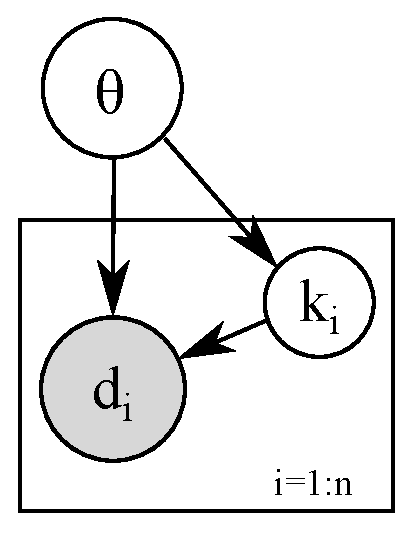
\includegraphics[width=0.2\textwidth]{pic/naive-mix2.pdf}
\caption{Mixture model Bayesian inference with parameter $\boldsymbol\theta$ and data points $d_1$ to $d_n$}
  \label{fig:naive.mix}
\end{figure}
%%%%%%%%%%%%%%%%%%%%%%%

%----------------------------------------***
\begin{proposition}
\label{pro:discrete}
Piecewise likelihood model $pr(d | \, \boldsymbol\theta)$ 
defined by relation~(\ref{e:piecewise.likelihood22}) is equivalent to 
$\sum_{k = 1}^N pr(k | \, \boldsymbol\theta) pr(d | \, k, \boldsymbol\theta)$
where:
\begin{equation}
\label{e:2rel22}
pr(k |\, \boldsymbol\theta) := 
{\footnotesize
\begin{cases}
\phi_k(\boldsymbol\theta)  &: 1\\
\neg \phi_k(\boldsymbol\theta) &: 0
\end{cases}
}%end font size
, 
\qquad 
pr(d | \, k, \boldsymbol\theta) := f_k(\boldsymbol\theta, d)
\end{equation}
%
\end{proposition}
\begin{proof}
Since constraints $\phi_k$ are mutually exclusive and jointly exhaustive: 
$$\sum_{k= 1}^N pr(k | \, \boldsymbol\theta) = 
\sum_{k=1}^N
{\footnotesize
\begin{cases}
\phi_k(\boldsymbol\theta)   &: 1\\
\neg \phi_k(\boldsymbol\theta)  &: 0
\end{cases}
}%end font size
\, =1
$$
Therefore $pr(k | \, \boldsymbol\theta)$ is a proper probability function. 
On the other hand, by marginalizing $k$, (\ref{e:2rel22}) trivially leads to (\ref{e:piecewise.likelihood22}):
\begin{align*}
\sum_{k} pr(k | \, \boldsymbol\theta)pr(d | \, k, \boldsymbol\theta) 
&= 
\sum_{k=1}^N  
{\footnotesize
\begin{cases}
\phi_k(\boldsymbol\theta)  &: 1\\
\neg \phi_k(\boldsymbol\theta) &: 0
\end{cases}
}%end font size
\, \cdot \, f_k(\boldsymbol \theta, d)
&&\text{by (\ref{e:2rel22})}
\\
&=
\sum_{k=1}^N 
{\footnotesize
\begin{cases}
		\phi_k(\boldsymbol\theta)  &: f_k(\boldsymbol\theta, d)\\
\neg 	\phi_k(\boldsymbol\theta)  &: 0
\end{cases}
}%end font size
= {\footnotesize
\begin{cases}
\phi_1(\boldsymbol\theta)  &: f_1(\boldsymbol\theta, d)\\
\vdots\\
\phi_n(\boldsymbol\theta)  &: f_N(\boldsymbol\theta, d)
\end{cases}
}%end font size
= pr(d | \, \boldsymbol\theta) 
&&\text{by (\ref{e:piecewise.likelihood22})}
\end{align*}
in which the third equality holds since constraints $\phi_k$ are mutually exclusive. 
\end{proof}
Proposition~\ref{pro:discrete} shows that a piecewise model can be converted  to a mixture model via augmenting it with auxiliary random variables. 
With a difference that the order of complexity of Gibbs sampling on the latter model is significantly less.
However, as the next subsection shows, it causes a \emph{deterministic dependencies problem} that should be addressed first.
 
%%take a single sample via Gibbs Let $\boldsymbol\theta := (\theta_1, \theta_2, \ldots, \theta_{|\boldsymbol\theta|})$. To take a sample from the posterior via Gibbs sampling on the original model (Fig.~\ref{fig:naive})  for each $i \in \{1, \ldots, |\boldsymbol\theta|\}$, $\theta_i$ should be sampled from $pr(\theta_j | \boldsymbol\theta_{-j}^*)$. As already shown, $pr(\theta_i | \, d_1, \ldots, d_n)  $ can consists of up to $MN^n$ partitions. $pr(\theta_i | \boldsymbol\theta_{-i}^*, \boldsymbol d)$ is the same function where all variables except one (i.e.\ $\theta_i$) are instantiated. Although this can reduce the number of feasible partitions, the upper bound on the number of partitions is still $MN^n$. In contrast, for Gibbs sampling on the model of Fig.~\ref{fig:naive.mix} Samples should be taken for (a) $pr(\theta_i | \boldsymbol\theta_{-i}^*, \boldsymbol k^*, \boldsymbol d)$ and  (b) $pr(K_j | \boldsymbol\theta^*, \boldsymbol k_{-j}^*, \boldsymbol d)$ where $\boldsymbol k_{-j}^*$ is the last taken samples for auxiliary random variables $\boldsymbol K := (K_1, \ldots, K_{j-1}, K_{j+1}, \ldots, K_n)$ that correspond observations $d_1$ to $d_n$ except $d_j$. In case (a), $\boldsymbol k^*$ determine a single combination of likelihood constraints $\theta$ (since only a single partition satisfies the constraints that corresponds to them). Even if conjunction of all $M$ prior constraints with such combination of such constraints is feasible, only $M$ partitions are produced. In case (b), $K_j$ is deterministically decided by $\boldsymbol\theta^*$ To put it short, the performance of Gibbs sampling on the aforementioned equivalent models significantly differs. Nonetheless, Gibbs sampling on the model augmented with auxiliary variables suffers from a problem that is going to be introduced and addressed in Sections~\ref{sect:deterministic} and \ref{sect:collapsed} respectively.  

\subsection{Deterministic dependencies problem}
\label{sect:deterministic}
%%%%%%%%%%%%%%%%%%%%%%%%%
\begin{figure}
  \centering
  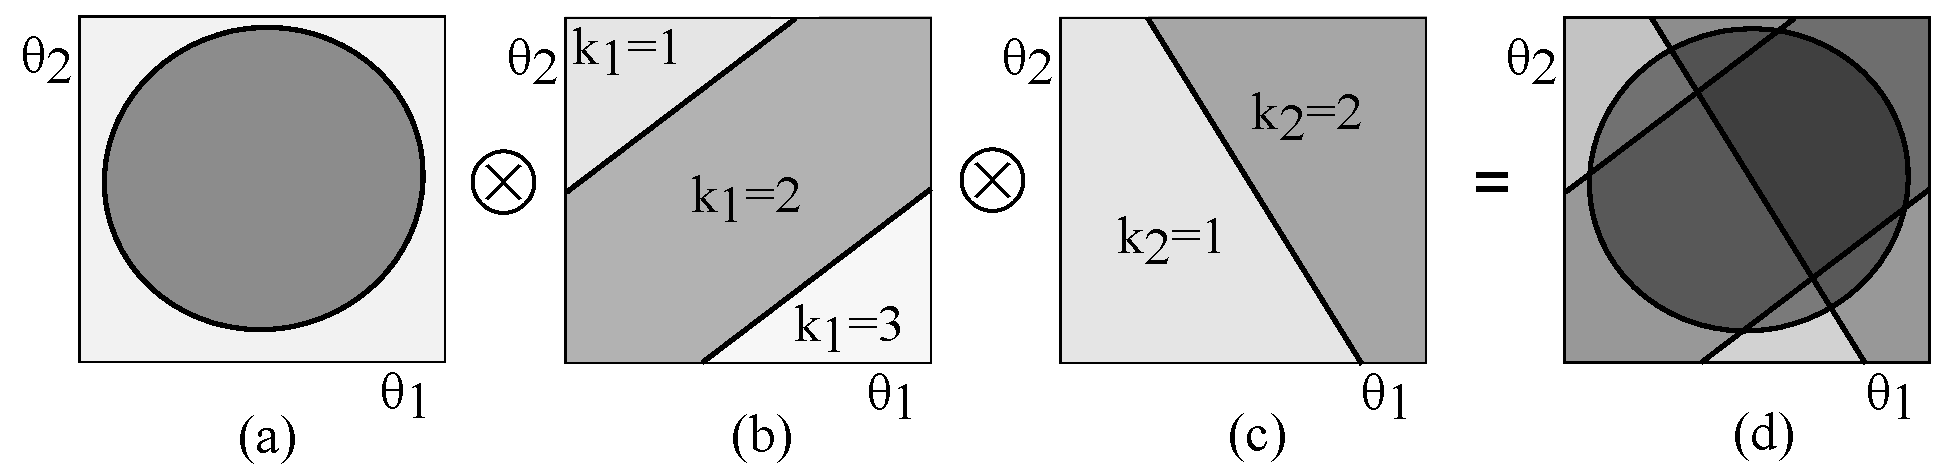
\includegraphics[width=0.95\textwidth]{pic/col21.pdf}
\caption{\footnotesize
A piecewise model with a 2-partitioned prior (a), 
a 2-partitioned and a 3-partitioned likelihoods (b \& c resp.) ending in a 12-partitioned joint/posterior distribution.
}
  \label{fig:simple.example}
\end{figure}
%%%%%%%%%%%%%%%%%%%%%%%

%%%%%%%%%%%%%%%%%%%%%%%%%
\begin{figure}
  \centering
  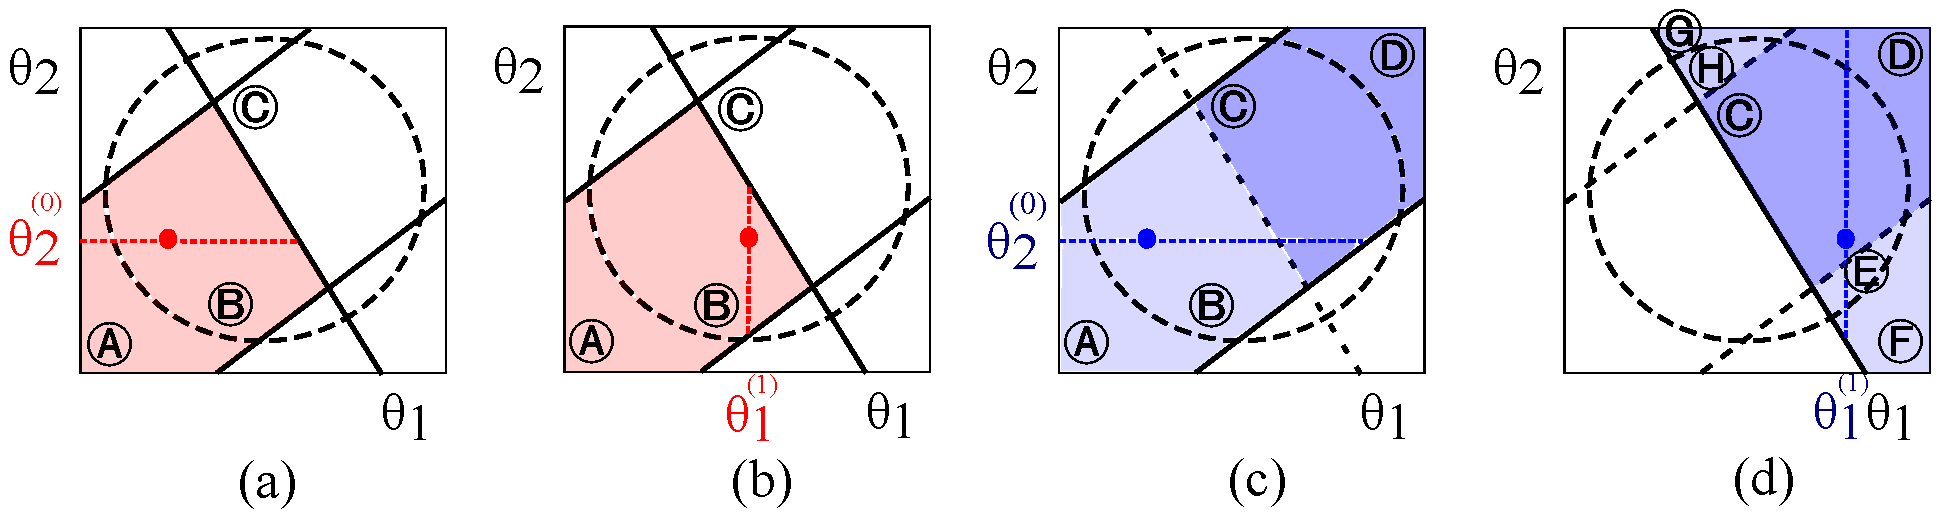
\includegraphics[width=0.95\textwidth]{pic/col22.pdf}
\caption{...}
  \label{fig:blocking}
\end{figure}
%%%%%%%%%%%%%%%%%%%%%%%
To illustrate the problem that emerges by Gibbs sampling on the mixture model defined by 
Proposition~\ref{pro:discrete}, consider the simple piecewise model depicted in 
Fig.~\ref{fig:simple.example} on a 2D parameter space 
$\boldsymbol\theta = (\theta_1, \theta_2)$ with a 2-piece prior, two observed points with a 2-piece and a 3-piece corresponding likelihood models. 
We augment the model by introducing auxiliary random variables $\bvec{k} = \{k_1, k_2\}$
such that $\textsc{Val}(k_1) = \{1,2,3\}$ and $\textsc{Val}(k_2) = \{1,2\}$ indicating (the constrain of) which partition in each likelihood function holds. 
Suppose Gibbs sampling is executed on the augmented model, starting from an initial point
$(\theta_1^{(0)}, \theta_2^{(0)}, k_1^{(0)} = 2, k_2^{(0)} = 1)$ 
(shown in Fig~\ref{fig:blocking}a as a filled red circle).
Firstly, $\theta$ is conditionally sampled:
$\theta_1^{(1)} \sim pr(\theta_1 | \, \theta_2^{(0)}, k_1^{(0)}, k_2^{(0)}) $ 
In Fig~\ref{fig:blocking}a, the interval on which 
this conditional distribution is non-zero is depicted with a red dashed line segment.
Clearly $\theta_1^{(1)}$ will be located inside partition (A) or (B) where 
$k_1 = 2$ and $k_2 = 1$ (i.e.\ second constraint of the first likelihood and the first constraint of the second likelihood function hold).
In the second step, $\theta_2$ is sampled (see Fig.~\ref{fig:blocking}b):
$\theta_2^{(1)} \sim pr(\theta_2 | \, \theta_1^{(1)}, k_1^{(0)}, k_2^{(0)})$ which again lies in either (A) or (B).
In the next step  
$k_1^{(1)} \sim pr(k_1 | \, \theta_1^{(1)}, \theta_2^{(1)}, k_2^{(0)})$ would deterministically take its former value $k_1^{(0)}$ since it is decided by $\boldsymbol\theta^{(1)}$.
Similarly, $k_2^{(1)} = k_2^{(0)}$. By following this process, it can clearly be seen that all generated particle(s) will remain in the union of partitions (A) and (B). 
This example reveals that Gibbs sampling on an augmented model is trapped in an initial set of partitions  
that specify the initial value of auxiliary variables).
A way round this problem is provided in the next subsection.  

%Let us clarify this problem by a simple example: Suppose in Example \ref{example:pref} items are single featured ($D = 1$), prior $pr(w) = \mathcal{U}(-1, 1)$, $\eta = 0.1$ and by a user response, item/feature $5$ is preferred over item/feature $6$. By relation (\ref{e:pref1likelihood}):
%\[
%pr(Q_1 = \textsc{First} | w, a_1 = 5, b_1 = 6) = 
%{\footnotesize
%\begin{cases}
%w<0: & 0.9\\
%w>0: & 0.1
%\end{cases}
%}%end footnote size
%\]
%Following Relation~\ref{e:2rel22} leads to relations~\ref{e:aaa1} and \ref{e:symptom}. After simplification, their cross product leads to relation~\ref{e:aaa3}: 
%\begin{equation}
%\label{e:aaa1}
%pr(K_1) = 
%{\footnotesize
%\begin{cases}
%K_1 = k_1: & 0.9\\
%K_1 = k_2: & 0.1 
%\end{cases}
%}%end footnote
%\end{equation}
%\begin{equation}
%\label{e:symptom}
%pr(Q_1 = \textsc{First} | K_1, w, a_1 = 5, b_1 = 6) =  
%{\footnotesize
%\begin{cases}
%K_1 = k_1: & 
%\begin{cases}
%w < 0: & 1\\
%w > 0: & 0 
%\end{cases}\\
%K_2 = k_2: & 
%\begin{cases}
%w < 0: & 0\\
%w > 0: & 1 
%\end{cases}
%\end{cases} 
%}%end footnote size
%\end{equation}
%\begin{equation}
%\label{e:aaa3}
%pr(w, K_1, \, Q_1 = \textsc{First}, a_1 = 5, b_1 = 6) \propto
%{\footnotesize
%\begin{cases}
%K_1 = k_1: & 
%\begin{cases}
%w < -1: & 0\\
%w < 0 \wedge w > -1: & 1\\
%w > 0: & 0 
%\end{cases}\\
%K_2 = k_2: & 
%\begin{cases}
%w < 0: & 0\\
%w > 0 \wedge w < +1: & 1 \\
%w> +1 : &0
%\end{cases}
%\end{cases} 
%}%end footnote size
%\end{equation}
%For Gibbs sampling from the posterior, let us start from an initial particle $(K_1^{(0)} = 2; w^{(0)} = 0.5)$ and sample from the joint distribution \ref{e:aaa3} for $K$ (while $w=0.5$ is instantiated). This ``deterministically" returns $K^{(1)}=2$ Now, we sample $w$ from the joint while instantiating $K_1 = 2$. This uniformly return a value in $\mathcal{U}(0, 1)$. Given such a value, $K_1^{(2)}$ would deterministically be 2 again, etc. So, in this example, Gibbs sampling never leave the region $K_1=2$.



\subsection{Blocked Gibbs sampling on mixture models}
\label{sect:collapsed}
To prevent the problem of deterministic dependencies, auxiliary variable are not sampled individually. 
Instead, at each step, a parameter variable $\theta_i$ is jointly sampled with  
(at least) one  
auxiliary variable $k_j$ 
conditioned on the remaining variables:
$
%\begin{equation*}
%\label{e:blocked1}
(\theta_i, k_j) \sim pr(\theta_i, k_j | \, \boldsymbol \theta_{-i}, \bvec{k}_{-j})  
%\end{equation*}
$
(\emph{blocked Gibbs sampling}).
This is done in 2 steps. In the first step, $k_j$ is marginalized over and $\theta_i$ is sampled (\emph{collapsed Gibbs sampling}):
$
\theta_i \sim \sum_{k_j} 
pr(k_j | \, \boldsymbol \theta_{-i}, \bvec{k}_{-j}) 
pr(\theta_i | \, k_j, \boldsymbol \theta_{-i}, \bvec{k}_{-j})  
$.
In the second step, $k_j$ is determined from $\boldsymbol \theta$:
$k_j = i \in \textsc{Val}(k_j)$ s.t.\ $\phi_i^j(\boldsymbol \theta) \equiv \top$
where $\phi_i^j$ is the $i$-th constraint of $j$-th likelihood function.
This trick is illustrated in Fig.~(\ref{fig:blocking}c) where $(\theta_1, k_2)$ are sampled jointly,
followed by joint sampling of $(\theta_2, k_1)$ in (in Fig.~\ref{fig:blocking}d). 
%where blocked Gibbs sampling of $\theta_1$ and $k_2$ 
%is followed by blocked sampling of $\theta_2$ and $k_1$.
%Firstly by marginalizing over $k_2$, a sample is taken from the intersection of (blue dotted) line $\theta_2 = \theta_2^{(0)}$ and the union of segments (A) \& (B) (where $K_2 = 1$) and segments (C) \& (D) (where $K_2 = 2$). 
%$pr(K_2 = 1 | \, \theta_2^{(0)})$ is non-zero on the left side of the line while the 
%$pr(K_2 = 2 | \, \theta_2^{(0)})$ is non-zero on its right side.   
%After sampling $\theta_1$ from the resulting univariate piecewise function 
%($\theta_1^{(1)}$ in Fig~\ref{fig:blocking}d),
%in the next step $\theta_2$ is jointly sampled with $K_1$...................................

Using this method, (at least for some combinations of auxiliary and parameter variables) deterministic dependencies does not occur. This prevents being trapped in a single subset of partitions.
What is remained is to provide of a systematic method to find auxiliary variables $k_j$ that, with a high  probability, are not determined by the other auxiliary variables, $\bvec{K}_{-j}$ when jointly sampled with a parameter variable $\theta_i$. 
%A desired $k_j$ should is crucial; otherwise sampling convergence would be slow.
%To prevent deterministic dependencies problem, the chosen $K_j$ should not be determined by other %variables $\boldsymbol \theta_{-i}, \bvec{K}_{-j}$. 
A key observation is that in a piecewise distribution,
the set of partitions satisfying the current valuation of $\bvec{k}$
often differs with its adjacent partitions in a single auxiliary variable.
Since such a variable is not determined by other variables, it can be used in the blocked sampling.\footnote{In case some likelihood functions share a same partitioning constraint, some adjacent partitions would differ in several auxiliary variables.
%would be duplicated and therefore deterministically dependent. 
%However, as long as such cases are not numerous sampling performance is not noticeably affected. %If such cases are not rare in the model, either such likelihood functions should be substituted with their product or 
in such cases, more than one auxiliary variable should be used for blocked sampling.
}%footnote   
To clarify this issue, in the example of Fig~(\ref{fig:blocking}a), consider finding a proper $k_j$ 
for joint sampling $pr(\theta_1, k_j | \, \theta_2^{(0)}, \bvec{k}_{-j}^*)$. It suffices to extend the red dotted line segment $pr(\theta_1 | \, \theta_2^{(0)}, \bvec{k}^*)$ in two sides to find a point in a neighboring partition e.g.\ (C) and return an auxiliary variable that differs between (C) and the union of (A) \& (B) which is $k_2$. This is exactly how, blocked sampling is carried out in Fig.~\ref{fig:blocking}. 
More generally, to find an auxiliary variable $k_j$ to be sampled jointly with a parameter variable $\theta_i$ conditioned on the other variables: 

1.  In the space of $\boldsymbol \theta$,
the variable assignment of two points not included in the line segment
$pr(\theta_i = \theta | \, \boldsymbol{\theta}_{-i}, \bvec{k})>0$ 
but adjacent to its ending points is computed: 
\begin{align*}
\theta_i^L := \inf   \{ \theta |\, p(\theta_i = \theta | \, \boldsymbol{\theta}_{-i}^*, \bvec{k}^*)>0 \} - \epsilon, \hspace{12mm}
\theta_i^U := \sup \{ \theta |\, p(\theta_i = \theta | \, \boldsymbol{\theta}_{-i}^*, \bvec{k}^*)>0 \} + \epsilon
\end{align*}
where $\epsilon>0$ is a very small number.

2. With probability 0.5, $\theta_i \leftarrow \theta_i^L$ otherwise $\theta_i \leftarrow \theta_i^U$.

3. The valuation of auxiliary variables determined by these bounds is obtained:
\begin{align*}
\hat{\bvec{k}} := (k_1, \ldots, k_m) \text{ s.t. } k_j \in \textsc{Val}(k_j),\, \phi^i_{k_j}(\theta) \equiv \top, \qquad \forall j \in \{1, \ldots, m\} 
\end{align*}
4. The set of auxiliary variables used in blocked sampling $(\bvec{k}^b, \theta_i)$ is the computed:
\begin{align*}
\bvec{k}^b = \{k_x \in \bvec{k} | \, k_x \neq \hat{k}_x\}
\end{align*} 

%\subsection{Order of complexity} Time/space complexity of Gibbs sampling on the two models differs significantly: To obtain a single particle via Gibbs sampling from a posterior $pr(\boldsymbol\theta | \, d_1, \ldots, d_n)$ on the original model (see Fig.~\ref{fig:naive}) in a parameter space $\boldsymbol\theta$ = $(\theta_1, \ldots, \theta_N)$, $N$ number of CDFs should be computed (one for each parameter $\theta_i$ while other parameters are instantiated). Therefore, up to $LM^nN$ integrations are required (where $L$ and $M$ are the the number of partitions in the prior and each likelihood respectively). In contrast, to take a particle on the model of Fig.~\ref{fig:naive.mix}, $N + n$, CDFs should be computed since the parameter space is augmented to $(\theta_1, \ldots, \theta_{N}, K_1, \ldots K_n)$ (where each auxiliary variable $K_i$ indicates what partition is ``activated" in $i$-th likelihood). Nonetheless, in the latter model, creation of CDFs is much less expensive: {\color{blue} The reason is that in a function $pr(\theta_i | \, \theta_{-i}^*, K_1^*, \ldots K_n^*)$ since auxiliary variables are instantiated, a single partition on each likelihood function is activated. By cross product of the activated partitions in the prior, a piecewise function with merely $L$  (rather than $LM^n$) partitions is created. }%color


\section{Experimental results}
\label{sect:experiment}

%To motivate the necessity for \emph{general piecewise models}, i.e.\ models in which prior/likelihood sub-functions are not necessarily constant, consider the following example:   
%%%%%%%%% MARKET MAKER
\vspace{1mm}
\fexample{example:market}{Market maker}{
To generalize the problem presented in \cite{Das:08}, 
assume there are $D$ different types of \emph{instruments} with 
respective valuations $v_{1}$ to $v_{D}$.
There is a \emph{market maker} 
that at each time step $t$, deals an instruments of type $\tau_t \in \{1, \ldots D\}$ by setting \emph{bid} and \emph{ask} prices $b_{t}$ and $a_{t}$ for it
at which he is willing to buy and sell one unit %(of type $\tau_t$) 
respectively 
(where $b_{t} \leq a_{t}$).
The ``true" valuation of different types %of instruments of a type $\tau^i$, $v_{\tau^i}$, 
is unknown (to the market maker) but any a priori knowledge over their dependencies that can be expressed via a DAG structure over their associated random variables is permitted.
Nonetheless, without loss of generality we only consider the following simple dependency:  
Let us assume the market maker knows that the valuation of instruments of type $1$, $v_1$, is in some given price range $[L, H]$ and instrument types are sorted according to their valuations 
(i.e.\ $v_{i} \leq v_{i+1}$) while the price difference of any pair of consecutive types is bound by a known parameter $\delta$:
\begin{equation*}
pr(v_{1}) = \mathcal{U}(L, H) \qquad \qquad
pr(v_{i+1}) = \mathcal{U}(v_{i}, v_{i} + \delta) \quad \forall i \in \{1, \ldots, D-1\}
\end{equation*} 
At each time-step $t$, a trader arrives. 
He has a noisy estimation $v_{t}^*$ of the actual value of the presented instrument $\tau_t$. 
We assume 
$pr(v_{t}^* | \, \bvec{v}, \, \tau_t = i) = \mathcal{U}(v_{i} - \epsilon, v_{i} + \epsilon)$
where $\bvec{v} := (v_{1}, \ldots, v_{D})$.
The trader response to bid and ask prices 
$a_{t}$ and $b_{t}$ is $Q_{t} \in \{\textsc{Buy}, \textsc{Sell}, \textsc{NoDeal}\}$. 
If he thinks the instrument is undervalued, with probability 0.8, he will buy it. 
If he believes that it is overvalued, with probability 0.1 he may still buy it (for reasons such as customers request, etc.):
\begin{equation}
pr ( Q_{t} \!=\! \textsc{Buy} \, | \, v_{t}^*, a_{t}, b_{t}) =
\begin{cases}
v_{t}^*  <     a_{t} 		: &0.1\\
v_{t}^*  \geq a_{t}  		: &0.8
\end{cases}
\end{equation}
If the trader thinks that the instrument is overvalued (or undervalued) with probability 0.8 (resp. 0.1) he will sell it:
\begin{equation}
pr ( Q_{t} \!=\! \textsc{Sell} \, | \, v_{t}^* , a_{t}, b_{t}) = 
%pr(Q_{a_t b_t} = \textsc{Sell} \, | \, v^*_t) =
\begin{cases}
v_{t}^* \leq b_{t} 		: &0.8\\
v_{t}^* > b_{t} 		: &0.1
\end{cases}
\end{equation}
Otherwise, the trader does not perform a deal:
%
\begin{equation}
pr ( Q_{t} \!=\! \textsc{NoDeal} \, | \, v_{t}^*, a_{t}, b_{t}) =
\begin{cases}
b_{t} < v_{t}^* < a_{t} 								 & : 0.8\\
v_{t}^* \leq b_{t} \, \vee\,  v_{t}^* \geq a_{t}	 	 & : 0.1
\end{cases}
\end{equation}
Based on traders' responses, the market maker wants to compute the posterior distribution of the valuations of all instrument types.
In order to transform this problem (with corresponding model shown in Fig.~\ref{fig:market})
to Bayesian inference model of Fig.~\ref{fig:naive}, variables $v_{t}^*$ should be marginalized.
For instance:
\begin{align*}
pr( Q_{t} \! = \! \textsc{Buy} \, | \, \bvec{v}, a_{t}, b_{t}, \tau_t) &= 
\int_{-\infty}^{\infty} pr( Q_{t} \! = \! \textsc{Buy} \, | \, v_{t}^*, a_{t}, b_{t})
\cdot pr (v_{t}^* \, | \, \bvec{v}, \tau_t ) d v_{t}^* \\
&= \int_{-\infty}^{\infty}
{\footnotesize
\begin{cases}
v_{t}^*  		<     a_{t}  : &0.1\\
v_{t}^*  		\geq a_{t}  : &0.8
\end{cases} 
}
\otimes
{\footnotesize
\begin{cases}
v_{\tau_t} - \epsilon \leq v_{t}^* \leq v_{\tau_t} + \epsilon 					: \frac{1}{2 \epsilon} \\
v_{t}^* < v_{\tau_t} - \epsilon \, \vee \, v_{t}^* > v_{\tau_t} + \epsilon 	: 0  
\end{cases}
}
d v_{t}^*\\
&=
%{\footnotesize
\begin{cases}
v_{\tau_t} > a_{t} + \epsilon : &0.8\\
a_{t} - \epsilon < v_{\tau_t} \leq a_{t} + \epsilon: &\frac{7 (v_{\tau_t} - a_{t})}{20 \epsilon} + \frac{9}{20}\\
v_{\tau_t} \leq a_{t} - \epsilon: &0.1
\end{cases}
%} footnote
\end{align*}
which is a piecewise polynomial rather than a piecewise constant.
}% end MM example
%%%%%%%%%%%%%%%%%%%%%%%%%
\begin{figure}%[t!]
\centering
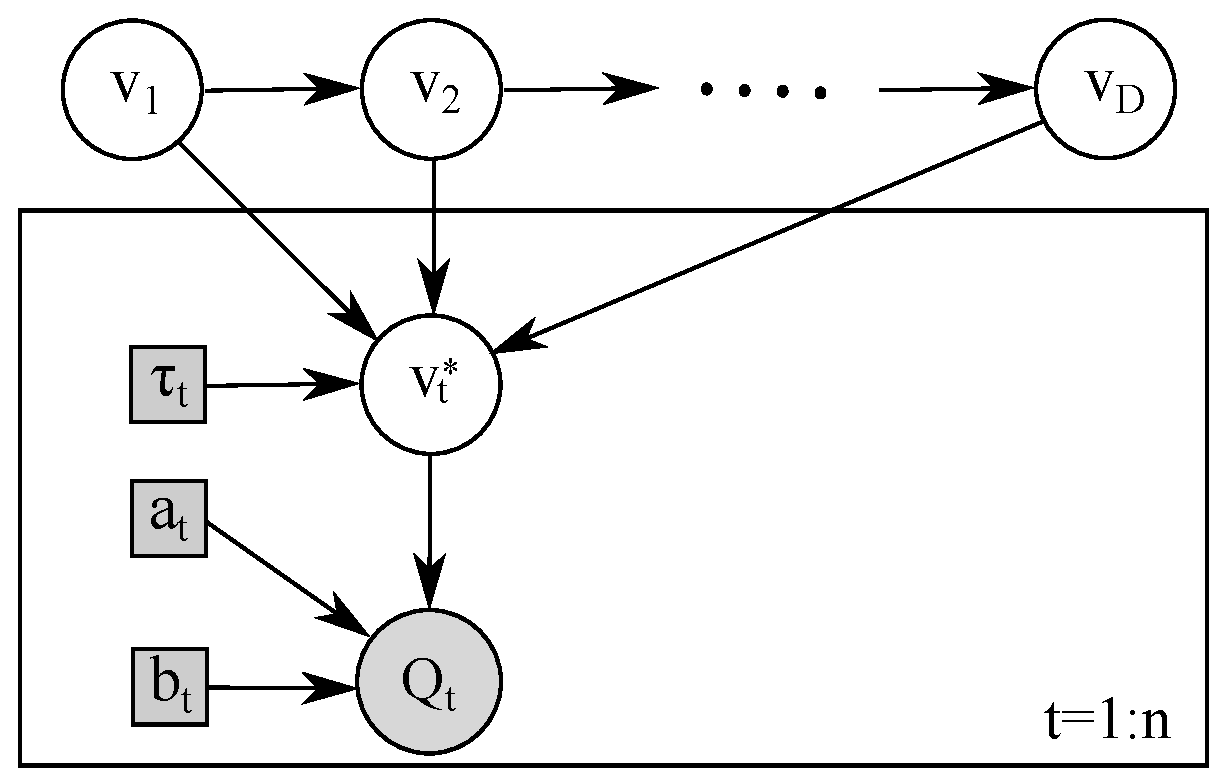
\includegraphics[width=.55\textwidth]{pic/market4.pdf}
%\vspace{-6mm}
\caption{\footnotesize Market maker model using plate notation. }
\label{fig:market}
%\caption{\footnotesize .} 
%\vspace{4mm}
\end{figure}
%%%%%%%%%%%%%%%%%%%%%%%%%
%%%%%%%%%%%%%%%%%%%%%%%%%
\begin{figure}
\centering
\begin{subfigure}{.36\textwidth}
  \centering
  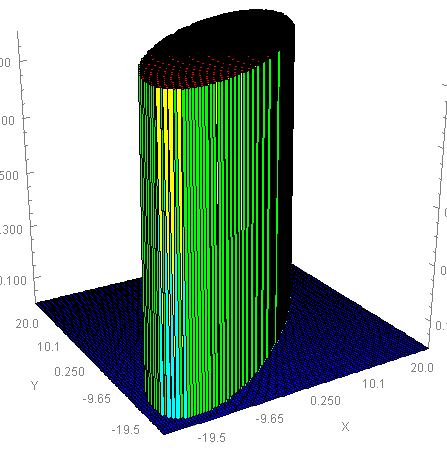
\includegraphics[width=.6\textwidth]{pic/elipsePrior.png}
  \caption{}
  \label{fig:mmm.prior}
\end{subfigure}%
\begin{subfigure}{.45\textwidth}
  \centering
  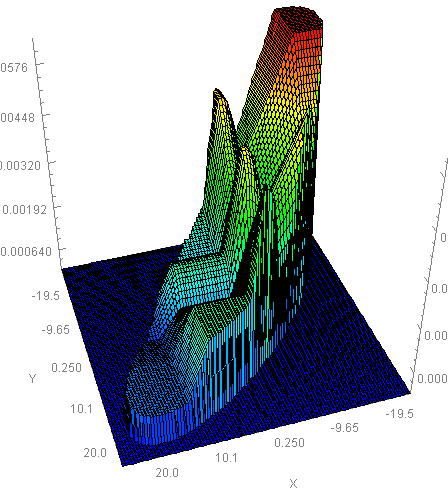
\includegraphics[width=.45\textwidth]{pic/MM2.png}
  \caption{}
  \label{fig:mmm.posterior}
\end{subfigure}
\caption{\footnotesize Instrument type value distribution of Market Maker problem of Example~\ref{example:market}.
(a) prior, (b) posterior given 4 observed data points (trader responses).}
\label{fig:mmm}
\end{figure}
%%%%%%%%%%%%%%%%%%%%%%%


.......................................



The main advantage of the proposed sampling method (on piecewise models) over baseline Gibbs sampling 
is that its order of growth vs.\ the amount of observed data is (at most) linear rather than exponential.
The price that we pay is to limit the next sample as being taken from a limited set of segments.
The question is how this effects the convergence rate of the sampling mechanism.
To answer this question, in this section we run the proposed algorithm along with other sampling methods on BPPL and MM models described in Examples~\ref{example:pref} and \ref{example:market}.
In BPPL problem we fix the dimension of the parameter space $\bvec{w}$ as 6.% and number of observed data as 10 (data points are chosen randomly). 
By taking 10,000 samples from the corresponding posterior
by means of \emph{rejection sampling} (as a baseline approach) we estimate the ground-truth mean of the parameter vector as $\hat{\bvec{w}}$.  
We generate 20 random queries $q_i = q_{a_i, b_i}$ where $1 \leq i \leq 20$
 and take the absolute difference between the predicted $u(a_i - b_i|\bvec{w})$ 
and the ground truth $u(a_i - b_i|\hat{\bvec{w}})$.
Subsequently, we compute the mean and \emph{standard error} of the obtained 20 values (as depicted in 
Figure~\ref{fig:results}).

%%%%%%%%%%%%%%%%%%%%%%%%%
\begin{figure}
\centering
\begin{subfigure}{.40\textwidth}
  \centering
  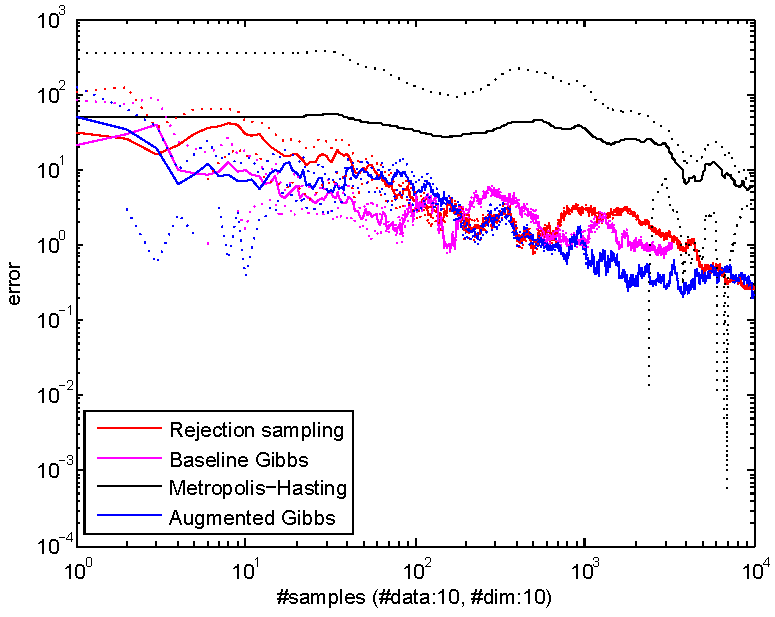
\includegraphics[width=1.00\textwidth]{pic/errVsamplesBPPL10.pdf}
  \caption{}
  \label{fig:error-samples-bppl}
\end{subfigure}
\begin{subfigure}{.40\textwidth}
  \centering
  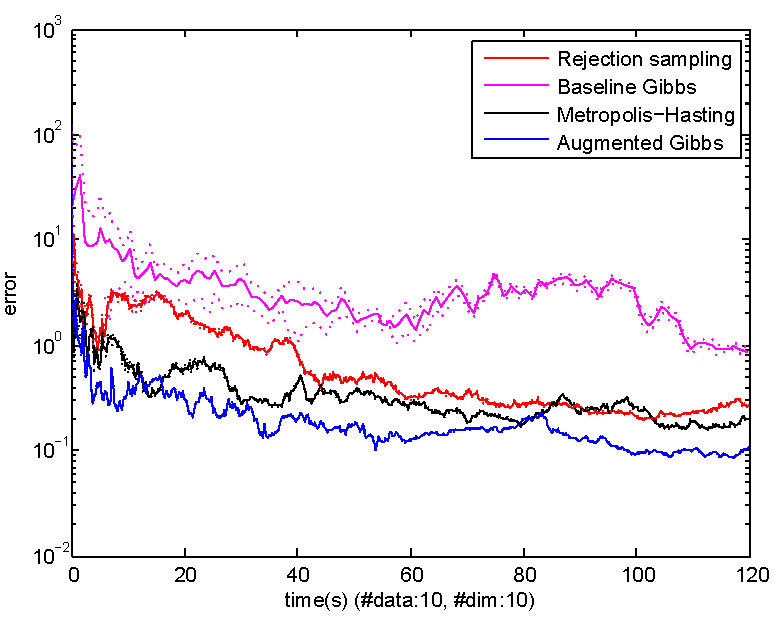
\includegraphics[width=1.00\textwidth]{pic/errVtimeBPPL10.pdf}
  \caption{}
  \label{fig:error-samples-bppl}
\end{subfigure}
\\%%%%%%%%%%%%%%%%%%%%%%%%%%
\begin{subfigure}{.40\textwidth}
  \centering
  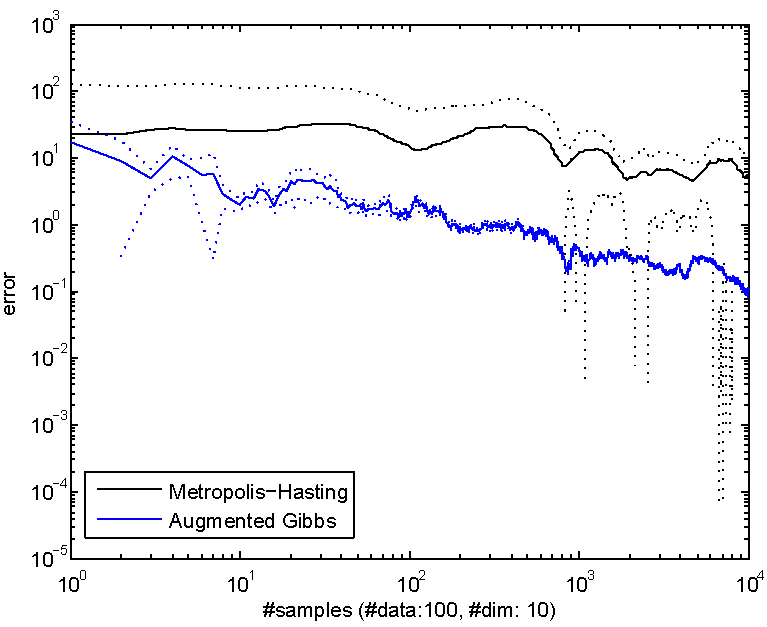
\includegraphics[width=1.00\textwidth]{pic/errorVSamplesBPPL-Big.pdf}%ERROR-VS-TIME FINAL-BPPL-BIG.pdf}
  \caption{}
  \label{fig:error-samples-bppl}
\end{subfigure}%
\begin{subfigure}{.40\textwidth}
  \centering
  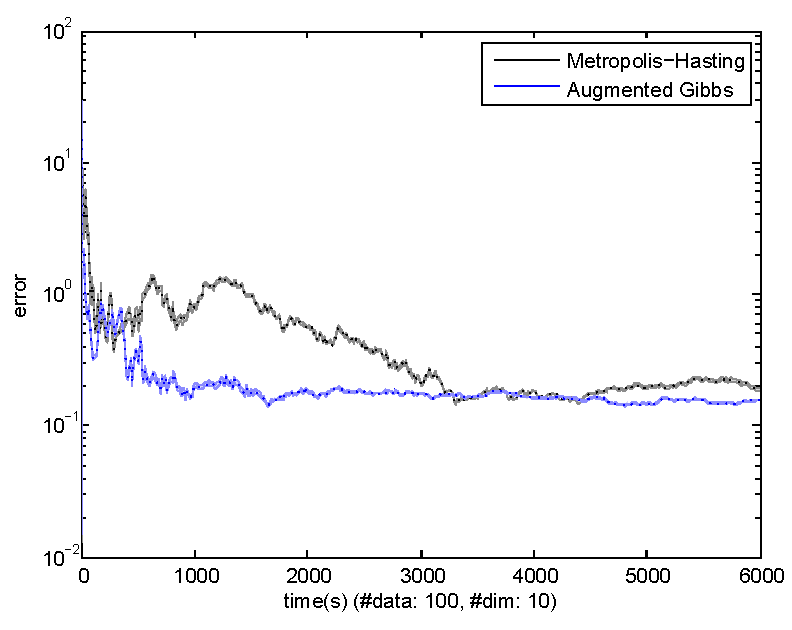
\includegraphics[width=1.05\textwidth]{pic/EVTBigBPPL.pdf}
  \caption{}
  \label{fig:error-samples-bppl}
\end{subfigure}%
\\
\begin{subfigure}{.40\textwidth}
  \centering
  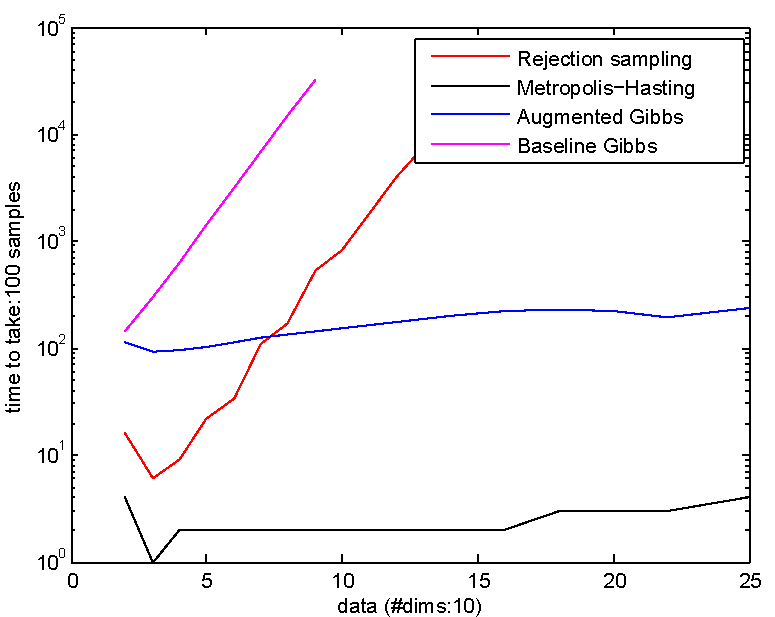
\includegraphics[width=1.05\textwidth]{pic/dim10analysis.pdf}%dims6-cnstrs10-time30000-q20-BPPL.png}
  \caption{}
  \label{fig:error-samples-bppl}
\end{subfigure}%
\caption{
\footnotesize
...%Experimental results. (a) error vs. no. taken samples (in a 30s time assigned to each algorithm) using rejection/augmented Gibbs (our work) and Metropolis-Hasting sampling algorithms for inference on the BPPL model in a 6 dimensional parameter space with 10 observed data points. (b) error vs. sampling time in the same setting. (c) time consumed to compute 10000 samples vs. different number of observed data. 
}
\label{fig:results}
\end{figure}
%%%%%%%%%%%%%%%%%%%%%%%
%%%%%%%%%%%%%%%%%%%%%%%%%
\begin{figure}
\centering
\begin{subfigure}{.40\textwidth}
  \centering
  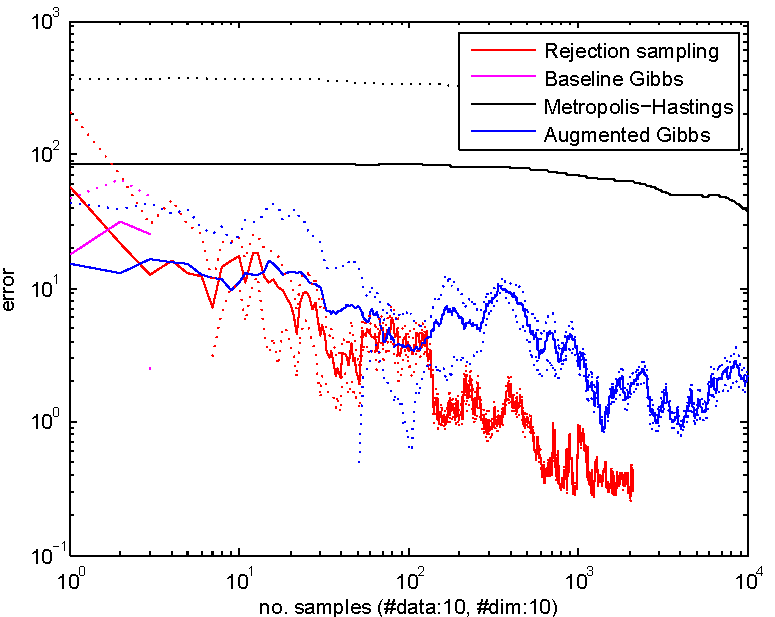
\includegraphics[width=1.00\textwidth]{pic/errVsamplesMMMdim10data10.pdf}
  \caption{}
  \label{fig:error-samples-bppl}
\end{subfigure}%
\begin{subfigure}{.40\textwidth}
  \centering
  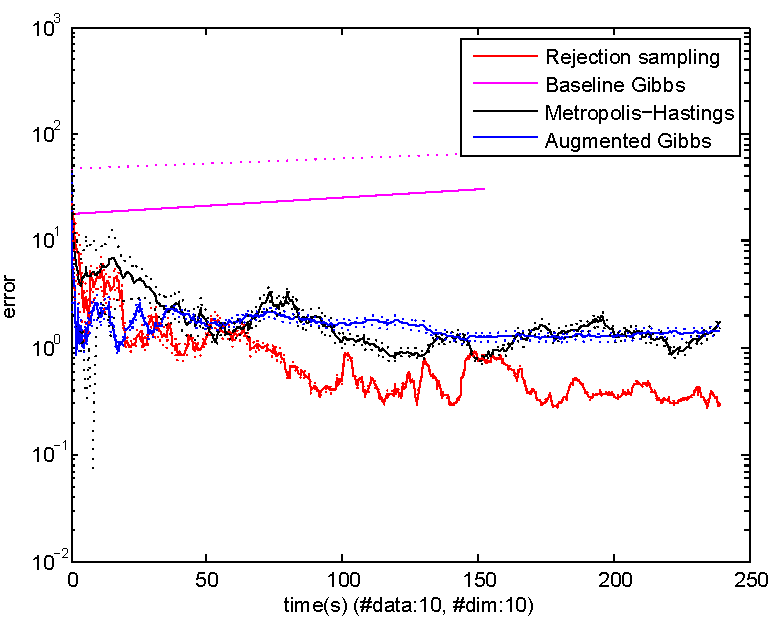
\includegraphics[width=1.05\textwidth]{pic/errVtimeMMMdim10data10.pdf}
  \caption{}
  \label{fig:error-samples-bppl}
\end{subfigure}%
\\
\begin{subfigure}{.40\textwidth}
  \centering
  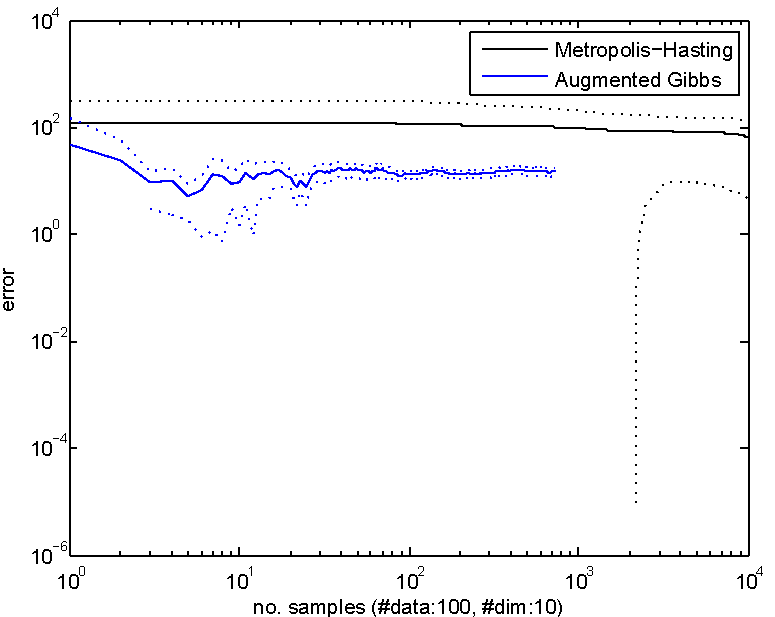
\includegraphics[width=1.00\textwidth]{pic/errVsamplesMMM100.pdf}
  \caption{}
  \label{fig:error-samples-bppl}
\end{subfigure}%
\begin{subfigure}{.40\textwidth}
  \centering
  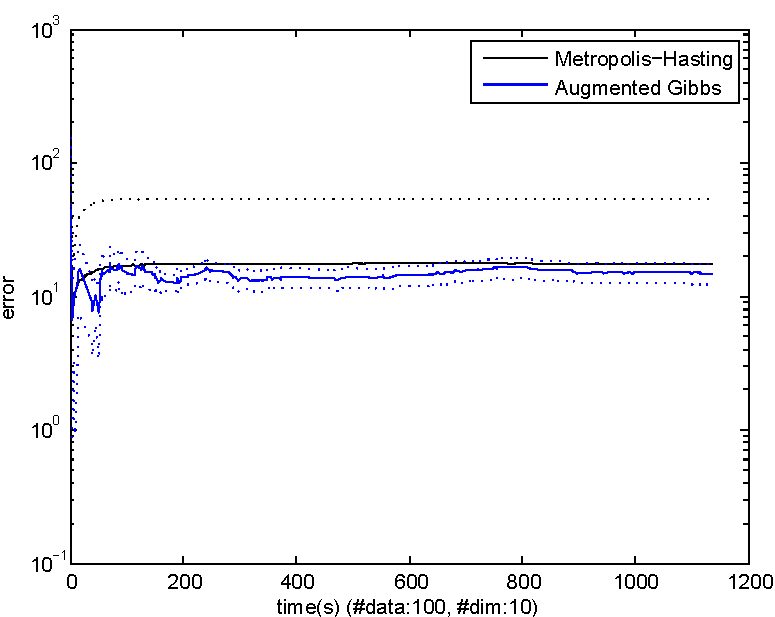
\includegraphics[width=1.05\textwidth]{pic/errVtimeMMM100.pdf}
  \caption{}
  \label{fig:error-samples-bppl}
\end{subfigure}%
\caption{
\footnotesize
...%Experimental results. (a) error vs. no. taken samples (in a 30s time assigned to each algorithm) using rejection/augmented Gibbs (our work) and Metropolis-Hasting sampling algorithms for inference on the BPPL model in a 6 dimensional parameter space with 10 observed data points. (b) error vs. sampling time in the same setting. (c) time consumed to compute 10000 samples vs. different number of observed data. 
}
\label{fig:results2}
\end{figure}




\begin{comment}
%%%%%%%%%%%%%%%%%%%%%%%%%
\begin{figure}
\centering
\begin{subfigure}{.40\textwidth}
  \centering
  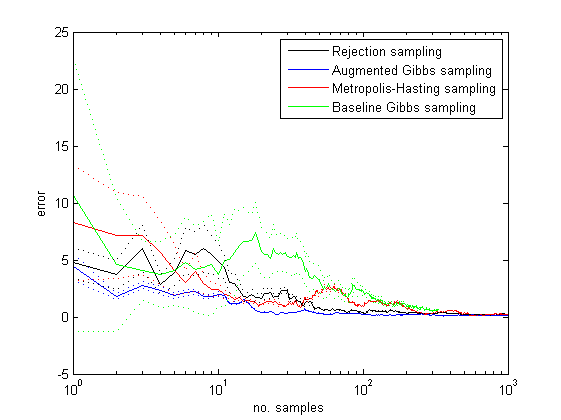
\includegraphics[width=1.05\textwidth]{pic/dim6cnstrs6-time30000-q20-MMM.png}
  \caption{}
  \label{fig:error-samples-mmm}
\end{subfigure}%
\begin{subfigure}{.40\textwidth}
  \centering
  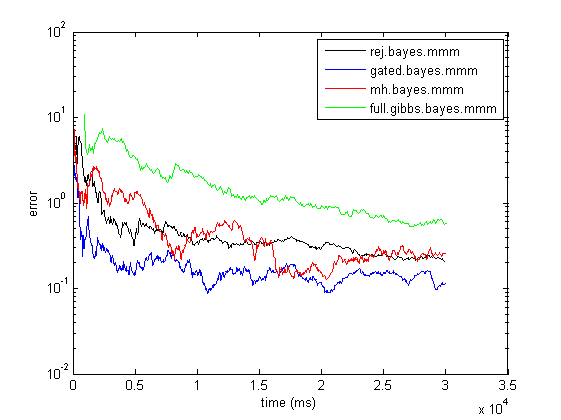
\includegraphics[width=1.05\textwidth]{pic/dim6cnstr6-time30000-q20-timeVsErrMMM-2.png}
  \caption{}
  \label{fig:error-time-mmm}
\end{subfigure}
\begin{subfigure}{.40\textwidth}
  \centering
  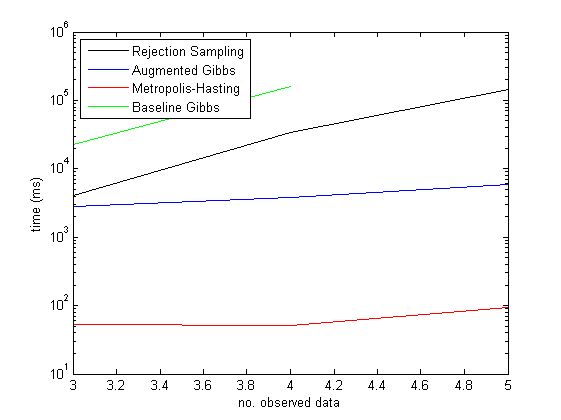
\includegraphics[width=1.05\textwidth]{pic/dim6variousConstraintsMMM.png}
  \caption{}
  \label{fig:data-points-effect}
\end{subfigure}%
%\begin{subfigure}{.45\textwidth}
 % \centering
  %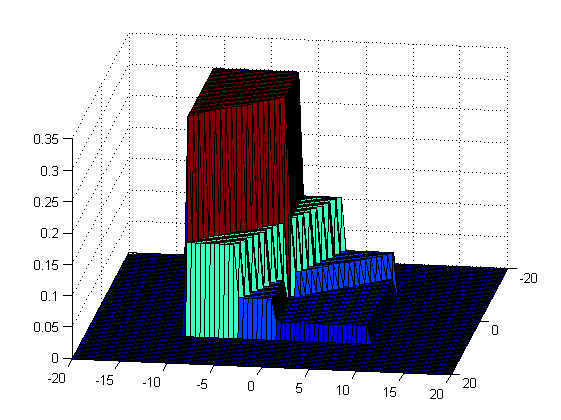
\includegraphics[width=.6\textwidth]{pic/posterior3d.png}
  %\caption{}
  %\label{fig:posterior3d}
%\end{subfigure}
\caption{
\footnotesize
Experimental results. (a) error vs. no. taken samples (in a 30s time assigned to each algorithm) using rejection/augmented Gibbs (our work) and Metropolis-Hasting sampling algorithms 
for inference on the BPPL model in a 6 dimensional parameter space with 10 observed data points.
(b) error vs. sampling time in the same setting.
(c) time consumed to compute 10000 samples vs. different number of observed data.
}
\label{fig:results}
\end{figure}
\end{comment}
%%%%%%%%%%%%%%%%%%%%%%%
\section{Conclusion}
Unlike rejection sampling and baseline Gibbs sampling, the proposed method does not grow exponentially with the amount of observed data.
In this sense its performance is much more similar to a typical MH sampling (such as the MH sampler with a Gaussian proposal distribution used in the experimental results).
Nonetheless, taking a single sample by means of a MH algorithm is typically much faster 
(See Figs.~\ref{fig:data-points-effect-bppl} and \ref{fig:data-points-effect}). 
Nonetheless in order to reach the stationary distribution and converge, MH requires taking much more samples (See Fig.~\ref{fig:error-samples-bppl} and \ref{fig:error-samples-mmm}).   
Finally (as Fig.~\ref{fig:error-time-bppl} and \ref{fig:error-time-mmm} illustrate) the experimental results show that the trade of is in favor of Augmented Gibbs sampling
{\color{red} is this a meaningful English sentence?} in the sense that it converges faster than all tested methods.
Furthermore MH suffers from two shortcomings:
\begin{itemize}
\item It relies on a tuning parameter and therefore is not fully automatic.
\item In order to converge it requires obtaining a huge amount of samples.
Although the sampling process itself might be fast, but saving/maintaining such a big data using it for computation can be costly.
\end{itemize}
The proposed algorithm, in contrast, is fully automatic and converges faster and with less amount of samples. Therefore, should be considered as a viable alternative to the existing asymptotically unbiased inference toolkit.



%\subsubsection*{References}
\small{
\bibliographystyle{alpha}%{plain}%{plainnat}  % needs package natbib
\bibliography{\jobname}       % uses \jobname.bib, according to \jobname.tex
}



\end{document}